
Because the production cross-section is substantially higher than the
$\WW$ cross-section, top backgrounds pose a significant challenge.
To reduce the top background, we introduce two top tagging methods.
Both methods rely on the fact that top quarks decay to $Wb$ with
almost certainty.

The first method vetoes events
containing soft muons from the $b$-quark decays.
The requirements used to select soft muons are:

\begin{itemize}
    \item $\pt > 3$ GeV;
    \item Reconstructed as a TrackerMuon
    \item Meets $\mathrm{TMLastStationAngTight}$ muon id requirements
    \item The number of valid inner tracker hits $>10$
    \item The transverse impact parameter with respect to the Primary Vertex, $|d_{0}| < 0.1$~cm,
    \item Non-isolated $({\rm{Iso}_{Total}}/{\pt}~>~0.1)$ if $\pt>20\GeV$.
\end{itemize}

The second method uses standard $b$-jet tagging.
In this method, events containing jets tagged with
 the $\mathrm{TrkCountingHighEff}$~\cite{btag} algorithm with
a discriminator value of greater than 2.1 are vetoed.
The algorithm is applied to jets with the same definition as Section \ref{sec:sel_jets},
with the exception that the $E_T$ requirement is removed. 
Thus, events in the zero-jet bin can still contain tagged jets.

The $\WW$ signal efficiency versus the $\ttbar$ efficiency in events with no jets according
to the definition in Section \ref{sec:sel_jets} for different standard b-tagging algorithms 
is shown in Figure~\ref{fig:eff_btag_tt_ww}. 
For a top rejection efficiency above $40\%$,
the $\mathrm{TrkCountingHighEff}$ tagger performs better than the others.
Our current cut value has a $\WW$ signal efficiency of about $98.1\%$ and
a $\ttbar$ efficiency of about $39\%$.

\begin{figure}[!htbp]
\begin{center}
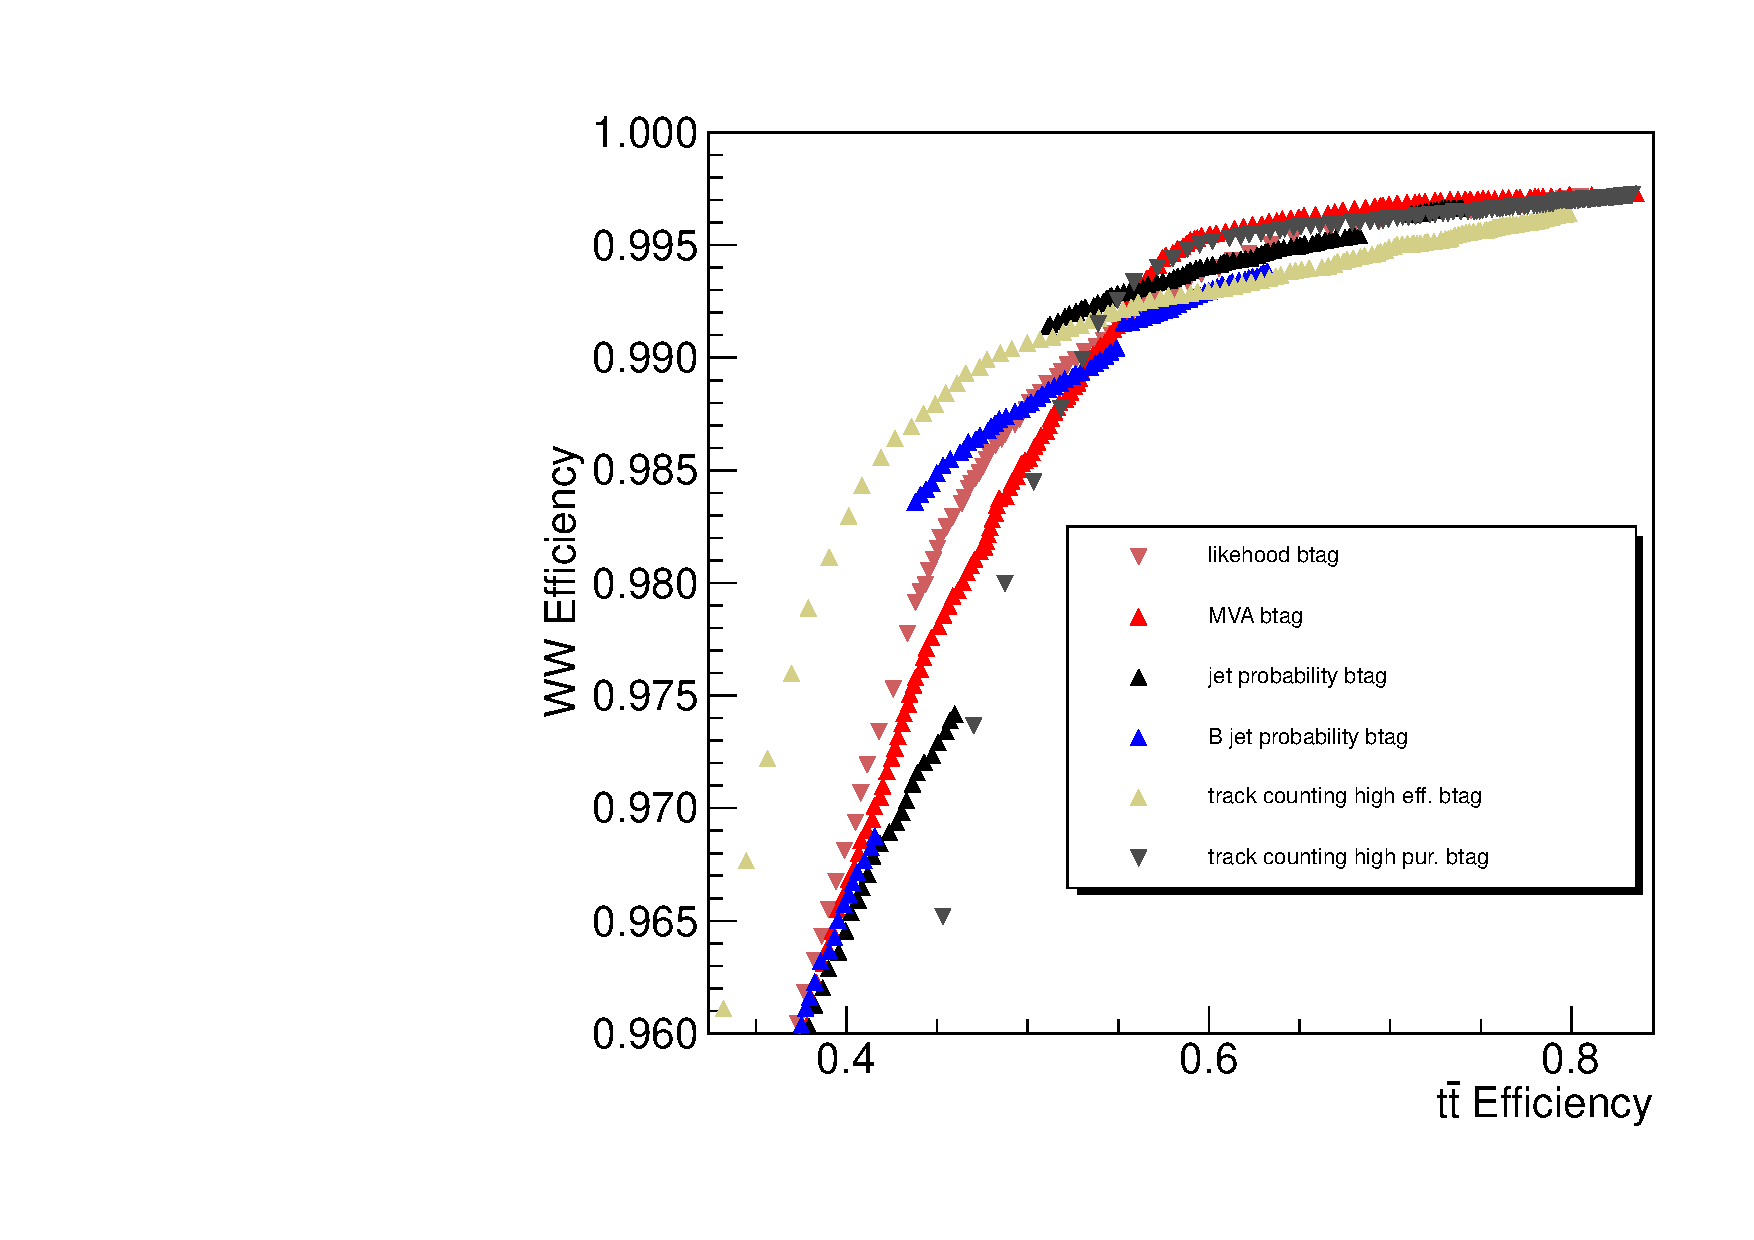
\includegraphics[width=0.60\textwidth]{figures/eff_btag_tt_ww.pdf}
\caption{$\WW$ signal efficiency versus $\ttbar$ efficiency in events with no
reconstructed jets for different standard b-tagging algorithms.}
\label{fig:eff_btag_tt_ww}
\end{center}
\end{figure}

By using the expected tagging efficiency for the two methods,
it is possible to estimate the residual top background after the vetoes
have been applied. This is described in detail in Section \ref{sec:bkg_top}.
